\section{Model Transformations}
\label{sec:slco:model-transformations}
Two types of model transformations are applied to transform \SLCO models to models or implementations in one of the target languages: endogenous transformations and exogenous transformations.
The input and output language of an endogenous model transformation is the same, whereas exogenous model transformations transform models from one language to another language~\cite{Mens:2006:TMT:1706639.1706924}.
The endogenous transformations are used to refine \SLCO models by bridging the semantic and platform gaps.
After all gaps have been bridged, the straightforward exogenous transformations can be applied.

\subsection{Endogenous Transformations}
\label{sec:slco:endogenous}
For each of the semantic gaps and platform gaps described in Section~\ref{sec:slco:language-gaps}, we implemented an endogenous model transformation that bridges this gap.
To keep these transformations simple, they can only be applied to models adhering to certain conditions.
In addition to the transformations that bridge the gaps, we implemented transformations that refine models to ensure that they adhere to the aforementioned conditions.

\subsubsection{Synchronized Communication over Asynchronous Channels}
\label{subsubsec:slco:sync2async}
To bridge the semantic gap between languages offering synchronous communication and languages that do not, we implemented two transformations.
Both transformations take an \SLCO model and a synchronous channel as input, and produce a model in which this channel is replaced by an asynchronous, lossless channel and the objects that communicate over this channel are adapted such that they communicate asynchronously.

\begin{figure}[hbt]
  \centering
  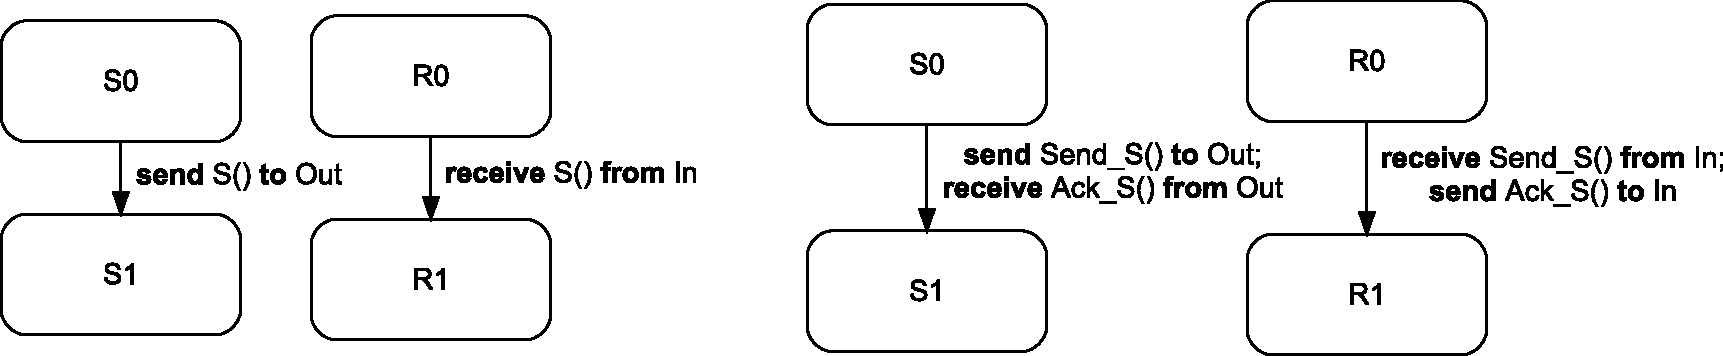
\includegraphics[scale=0.45]{slco/figs/transformations/s2a_simple}
  \caption{State machines before and after applying the simple version of \Transformation{as}}
  \label{fig:slco:trans:assimple}
\end{figure}

The first transformation is simple, but can only be applied to models that do not contain states with multiple outgoing transitions if one of these transitions starts with a statement that sends a signal over the synchronous channel.
The transformation ensures that the behavior of the model is still as desired by adding acknowledgment signals for synchronization.
Whenever a signal is sent, the receiving party sends an acknowledgement indicating that the signal has been received.
The sending party waits until it receives this acknowledgement.
In this way, synchronization is achieved.
On the left of Figure~\ref{fig:slco:trans:assimple}, two partial state machines are shown that send and receive a signal~\SLCOSignalName{S}.
Initially, ports~\SLCOPort{In} and~\SLCOPort{Out} are connected by a synchronous channel.
After transformation, acknowledgements are added, as shown on the right of the figure, and the synchronous channel is replaced with an asynchronous, lossless channel.
This transformation is described in more detail in Appendix~\ref{ap:transformations-slco}, and its correctness is discussed in Chapter~\ref{chap:reusable-correct-transformations} and Appendix~\ref{ap:proof}.

\begin{figure}[hbt]
  \centering
  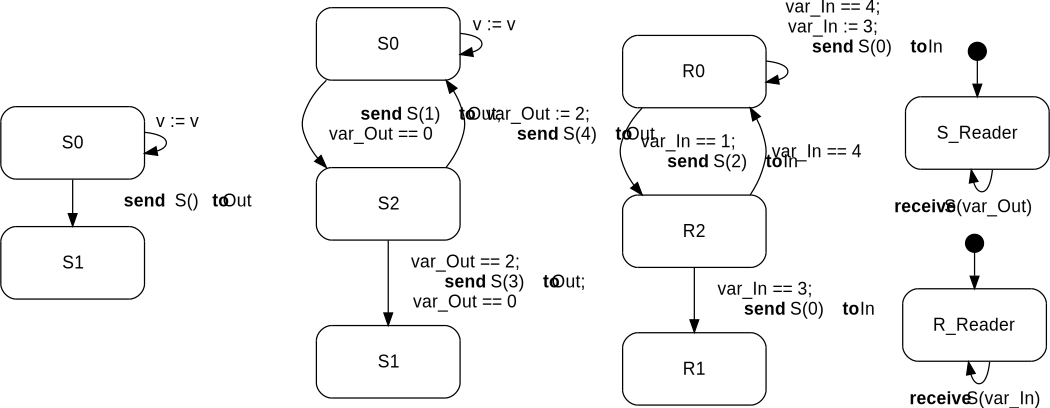
\includegraphics[scale=0.45]{slco/figs/transformations/s2a_complex}
  \caption{State machines before and after applying the general version of \Transformation{as}}
  \label{fig:slco:trans:ascomplex}
\end{figure}

The second transformation can be applied to any \SLCO model, but is more complex.
The partial state machine on the left of Figure~\ref{fig:slco:trans:ascomplex} shows an example of a situation where the transformation described above cannot be applied.
State~\SLCOState{S0} has multiple outgoing transitions, and one of these transitions starts with a statement that sends a signal.
In such situations, a more complex protocol has to be applied to ensure that the behavior of the model before and after transformation is the same, apart from the communication over the channel that is replaced.
Also in this example, ports~\SLCOPort{In} and~\SLCOPort{Out} are initially connected by a synchronous channel, which is replaced by an asynchronous, lossless channel.
In Figure~\ref{fig:slco:trans:ascomplex}, the second partial state machine from the left shows how the sending state machine is affected by the transformation, and the third partial state machine from the left shows how the receiving state machine is affected.
Additionally, two other state machines are added to the model, which are shown on the right of Figure~\ref{fig:slco:trans:ascomplex}.
State machine~\SLCOStateMachine{S\_Reader} is added to the object that sends signals, and state machine~\SLCOStateMachine{R\_Reader} is added to the object that receives signals.
Together with these state machines, the sender and receiver implement a protocol that ensures that states~\SLCOState{S1} and~\SLCOState{R1} are only reached if the communication between the sender and receiver was successful.
Furthermore, as long as the sender and receiver are unable to communicate, all enabled outgoing transitions of states~\SLCOState{S0} and~\SLCOState{R0} can be made.
Appendix~\ref{ap:transformations-slco} provides a more detailed description of this transformation.

The protocol that is employed by this transformation is not straightforward.
Therefore, we used the state-space generator for \SLCO described in Chapter~\ref{chap:prototype-semantics} for feedback during its development.
Informally, the protocol consists of the following steps.
Initially, the value of variable~\SLCOVariable{var\_Out} is equal to~0, and the value of variable~\SLCOVariable{var\_In} is equal to~3.
First, the sending object sends a signal~\SLCOSignal{S}{1} to indicate that it wants to communicate.
It can proceed to state~\SLCOState{S2} if all previous signals have been acknowledged by the receiving object, which is the case if variable~\SLCOVariable{var\_Out} is equal to~0.
The signal sent by the sending object is received by state machine~\SLCOStateMachine{R\_Reader}, and the value of its argument is stored in~\SLCOVariable{var\_In}.
Once the receiving object is informed of the intent of the sending object by means of the execution of statement~$\SLCOVariable{var\_In}==1$, it sends a signal~\SLCOSignal{S}{2} to indicate that it is ready to communicate.
Once this signal has been received and the value of its argument has been stored in variable~\SLCOVariable{var\_Out} by state machine~\SLCOStateMachine{S\_Reader}, the sending object may choose to complete the communication by sending signal~\SLCOSignal{S}{3}.
Alternatively, it may choose to cancel the communication by sending signal~\SLCOSignal{S}{4}.
Upon receiving one of these signals, the receiving object can take the transition to state~\SLCOState{R1} if the communication has been completed successfully, or take the transition to state~\SLCOState{R0} if it has been canceled.
Either way, it acknowledges the reception of the signal of the sending object by sending a signal~\SLCOSignal{S}{0}.
The state machines~\SLCOStateMachine{S\_Reader} and~\SLCOStateMachine{R\_Reader} ensure that the statements that send signals cannot be blocked, by emptying the buffers associated to the channels continuously.
It is possible that the sending object sends signal~\SLCOSignal{S}{4} after sending signal~\SLCOSignal{S}{1}, while the receiving object remains in state~\SLCOState{R0}.
The self-loop on state~\SLCOState{R0} ensures that an acknowledgement is also sent in this situation.

In the remainder, the simple version of this transformation is referred to as~\TSim, and the general version is referred to as~\TGen.
In cases where it is not relevant which of these two transformations is applied, the abbreviation~\Transformation{as} is used.

\subsubsection{Lossless Communication over a Lossy Channel}
\label{subsubsec:slco:ll}

Transformation~\Transformation{ll} implements lossless communication over a lossy channel by introducing auxiliary objects that implement a concurrent version of the Alternating Bit Protocol~(ABP)~\cite{Bartlett1969} known as the Concurrent Alternating Bit Protocol (CABP)~\cite{Baeten2002}.
This transformation is only applicable to unidirectional channels that are used to communicate signals named \SLCOSignalName{Signal} and whose only argument is a string.

\begin{figure}[hbt]
  \centering
  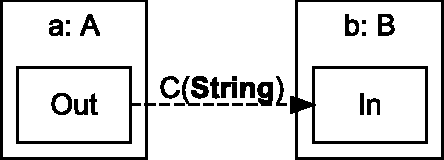
\includegraphics[scale=0.45]{slco/figs/transformations/Communication_Lossless2Lossy}
  \caption{Two objects communicating over an asynchronous, lossless channel}
  \label{fig:slco:ll-comm-before}
\end{figure}

Figure~\ref{fig:slco:ll-comm-before} shows a model consisting of two objects~(\SLCOObject{a} and~\SLCOObject{b}) that communicate over an asynchronous, lossless channel~(\SLCOChannel{C}).
After transformation, channel~\SLCOChannel{C} is replaced by the channels~\SLCOChannel{c1} to~\SLCOChannel{c6} and four objects that implement the CABP, as shown in Figure~\ref{fig:slco:ll-comm-after}.
Object~\SLCOObject{a} is connected to an object named~\SLCOObject{sender}, which communicates over an asynchronous, lossy channel~\SLCOChannel{c2} with an object named~\SLCOObject{receiver}.
The object named~\SLCOObject{receiver} is in turn connected to the object~\SLCOObject{b}.
After transformation, objects~\SLCOObject{a} and~\SLCOObject{b} communicate with each other via the aforementioned objects, instead of directly.
Objects~\SLCOObject{a} and~\SLCOObject{b} are connected to these objects by synchronous channels.
After receiving a signal from object~\SLCOObject{a}, object~\SLCOObject{sender} repeatedly sends this signal over channel~\SLCOChannel{c2} until it receives an acknowledgement from object~\SLCOObject{ar}, to which it is connected via the synchronous channel~\SLCOChannel{c6}.
After receiving a signal over channel~\SLCOChannel{c2}, object~\SLCOObject{receiver} forwards this signal to object~\SLCOObject{b} and instructs object~\SLCOObject{as} to continuously acknowledge the reception of this signal.
Object~\SLCOObject{as} does this by continuously sending signals over the asynchronous, lossy channel~\SLCOChannel{c5}.
The acknowledgement sent by object~\SLCOObject{as} contains a two-valued argument that is used by object~\SLCOObject{ar} to assess whether a particular acknowledgement signal was already received before.
Once object~\SLCOObject{ar} has received a new acknowledgement, it notifies object~\SLCOObject{sender}.
After receiving such a notification, object~\SLCOObject{sender} is able to receive a new signal from object~\SLCOObject{a} and transmit this signal over channel~\SLCOChannel{c2}.

In Figure~\ref{fig:slco:cabp}, the four state machines are shown that specify the behavior of the four objects that implement the CABP.
To show which state machine is part of which class, the names of the states have been chosen such that they reflect the names of the classes and objects.

\begin{figure}[hbt]
  \centering
  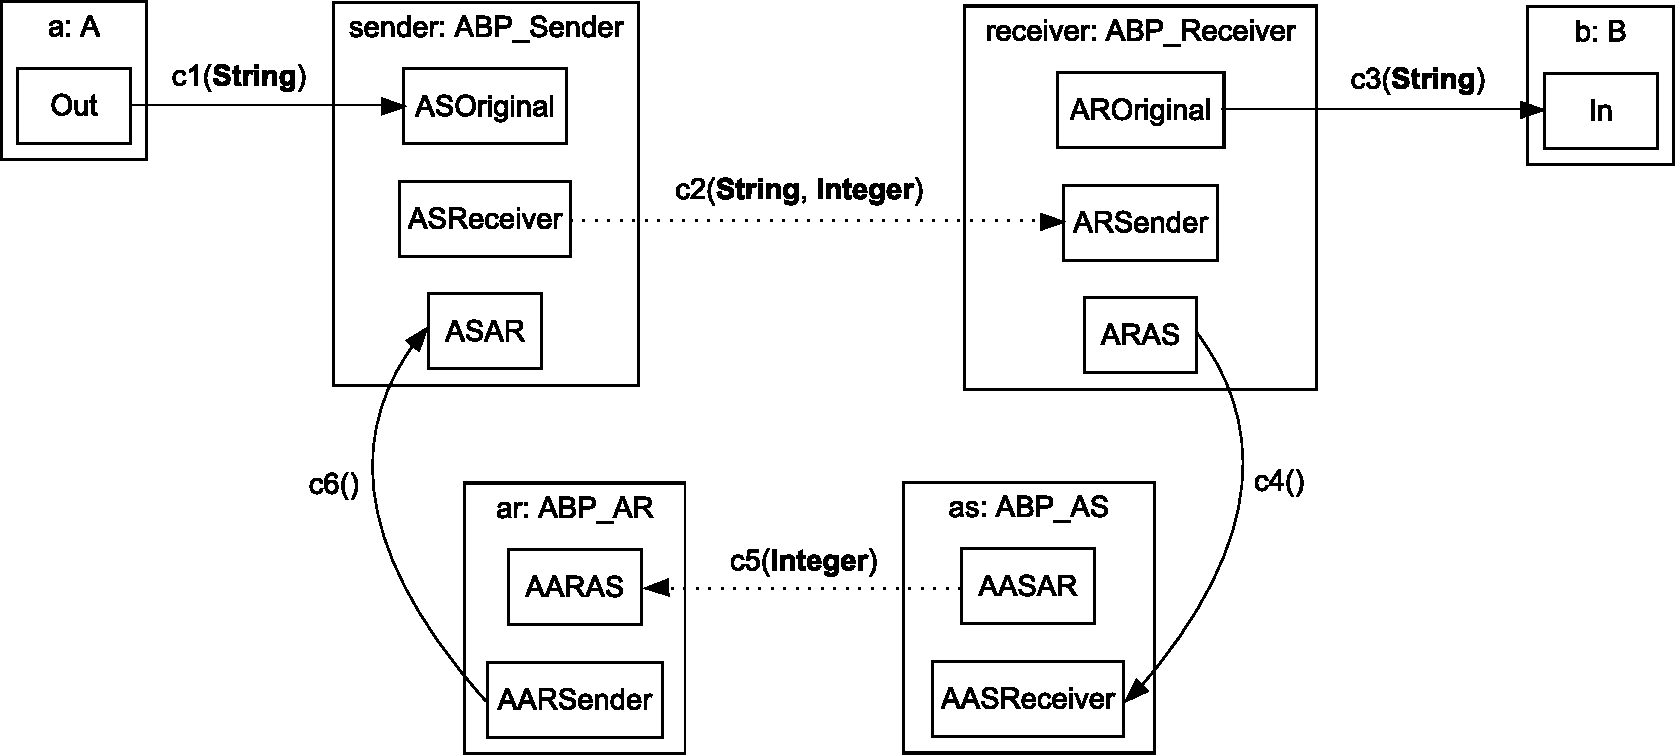
\includegraphics[scale=0.45]{slco/figs/transformations/Communication_Lossless2Lossy_ll}
  \caption{Two objects that communicate via the CABP}
  \label{fig:slco:ll-comm-after}
\end{figure}



\begin{figure}[hbt]
  \centering
  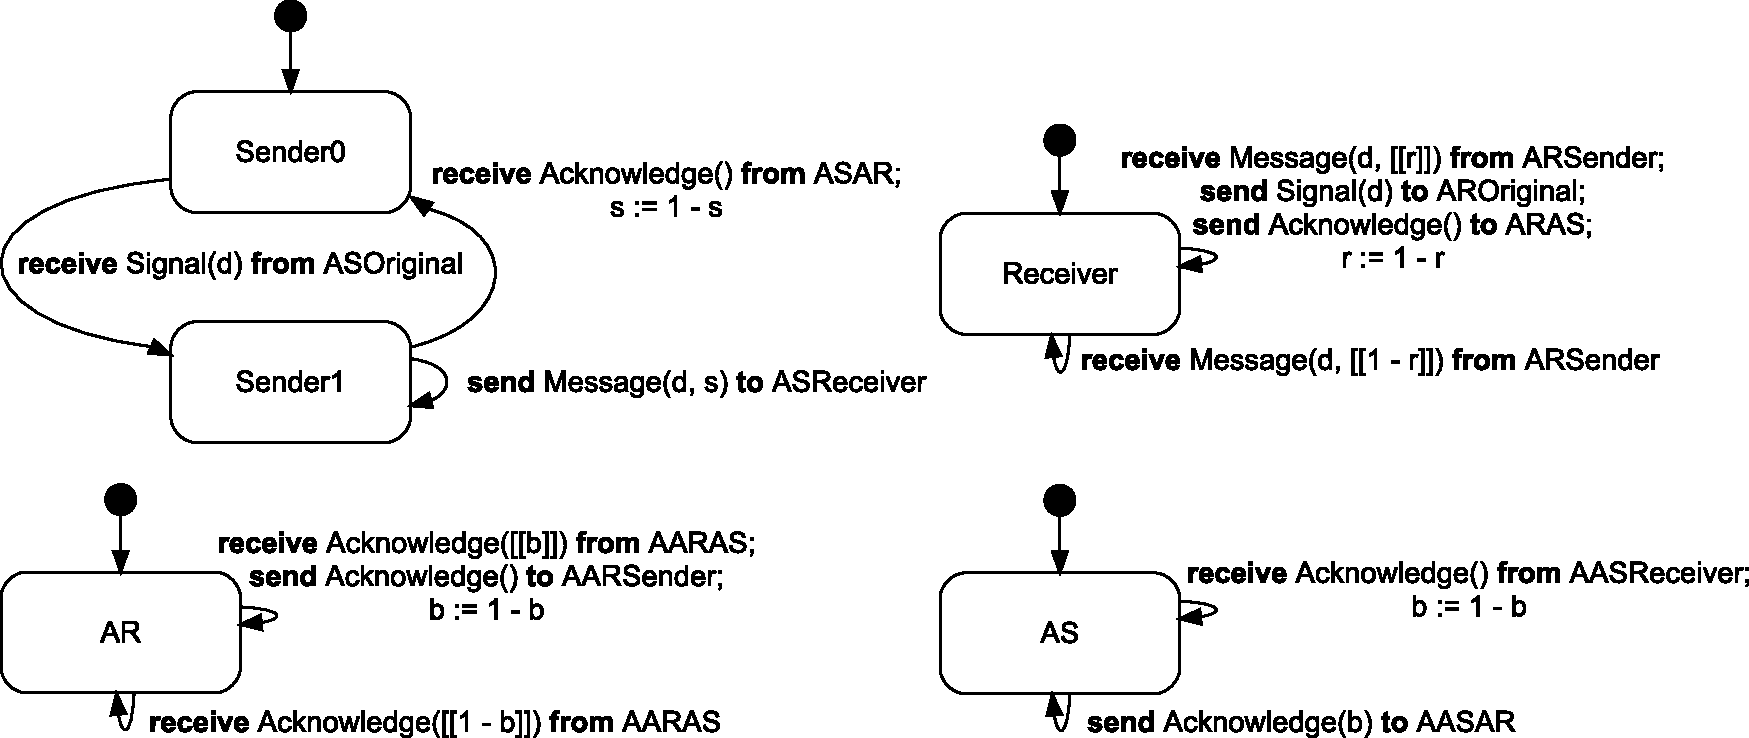
\includegraphics[scale=0.45]{slco/figs/transformations/ABP}
  \caption{Four state machines implementing the CABP}
  \label{fig:slco:cabp}
\end{figure}

\subsubsection{Adding Delays to Transitions}
Transformation~\Transformation{time} takes a model and a set of transitions as input, and adds delay statements to these transitions.
This transformations is used to control the frequency of the acknowledgments sent by the objects implementing the CABP.
Because it reduces the number of signals that are sent, it also reduces the number of collisions between messages sent via infrared on the Lego Mindstorms platform.

%%%

\subsubsection{Replacing Strings by Integers}
Transformation~\Transformation{int} replaces each string constant in an \SLCO model with a unique integer constant and changes the type of all string variables and arguments to integer.
This transformation deals with the fact that \NQC does not offer strings.

\subsubsection{Making the Sender of a Signal Explicit}
When multiple objects broadcast signals with the same name and number of arguments over the same medium, the receiving object cannot determine the origin of such a signal.
This situation arises when multiple \RCX controllers communicate with each other, because they communicate by broadcasting messages via infrared.
To enable a receiving controller to determine the origin of each signal it receives, transformation~\Transformation{ic} can be applied to a model.
This transformation takes a model and a set of channels as input, and adds an index to all signal names that identifies the channel over which these signals are sent.

\subsubsection{Reducing the Number of Objects}
\label{subsubsec:slco:merge}
Transformation~\Transformation{merge} merges multiple objects into one object.
Given a model and a set of objects, it creates a new object that contains all the variables, ports, and state machines contained by the objects provided as input.
By reducing the number of objects in a model, it bridges the corresponding gap between \SLCO and \NQC.
If any of the objects that are being merged communicate over synchronous channels, then this form of communication is replaced by communication using shared variables.
Transformation~\Transformation{merge} is only applicable to objects that satisfy the following condition: each pair of state machines that are part of two communicating objects must communicate over a unique unidirectional, synchronous channel.

\begin{figure}[hbt]
  \centering
  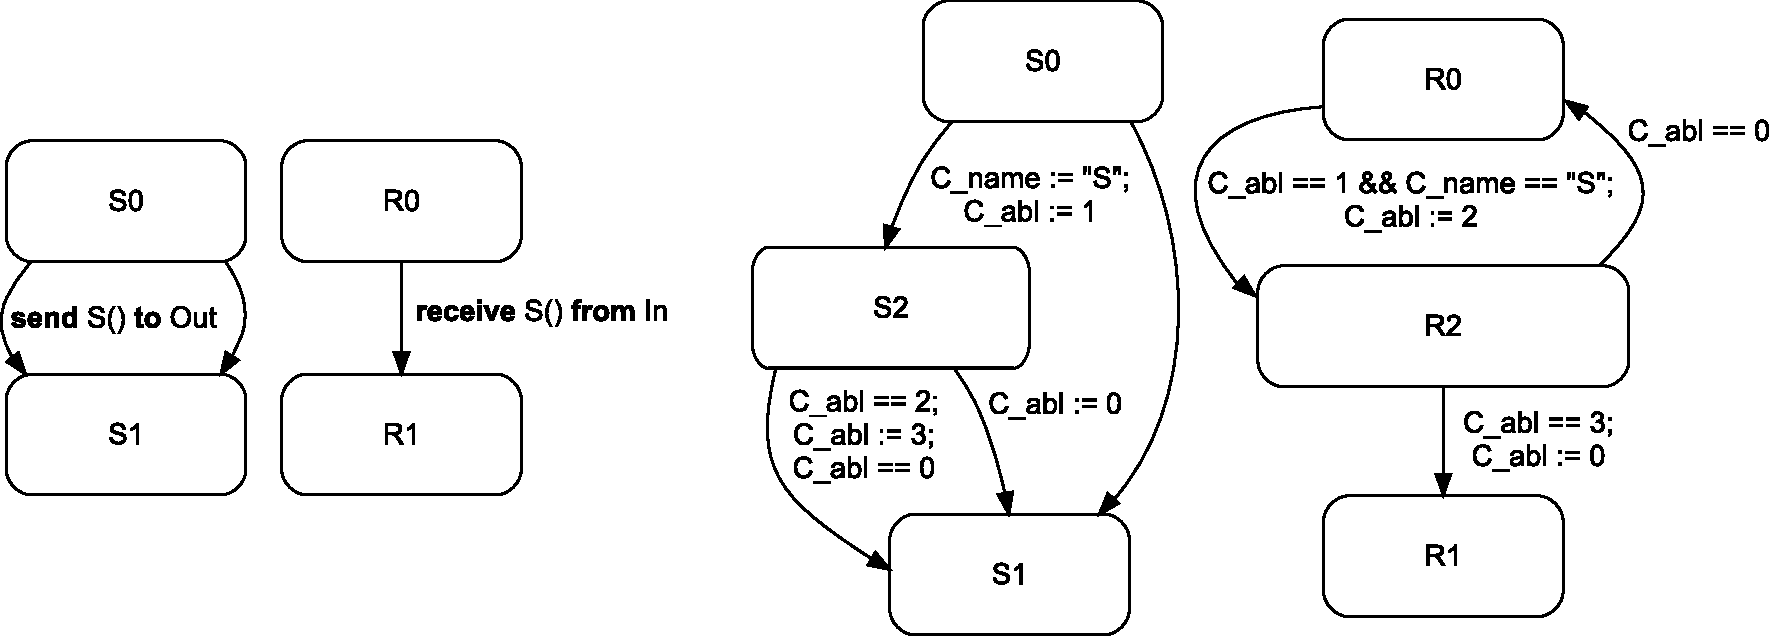
\includegraphics[scale=0.45]{slco/figs/transformations/MergeObjects}
  \caption{Two state machines before and after merging objects}
  \label{fig:slco:merge}
\end{figure}

Figure~\ref{fig:slco:merge} shows how communication over a synchronous channel is replaced by communication using shared variables.
The two partial state machines on the left of the figure are part of two separate objects and communicate with each other by sending and receiving signals over a synchronous channel that connects ports~\SLCOPort{In} and~\SLCOPort{Out}.
After merging these two objects, the state machines are adapted as shown on the right of the figure and communicate using the shared variables~\SLCOVariable{C\_name} and~\SLCOVariable{C\_abl}.
Variable~\SLCOVariable{C\_name} is used to store and retrieve the names of the signals that are being exchanged, and variable~\SLCOVariable{C\_abl} encodes the states of the employed communication protocol.
The sending state machine sets the value of~\SLCOVariable{C\_abl} to~1 to indicate that it wants to communicate.
The receiving state machine indicates that it is also able to communicate by setting the value of~\SLCOVariable{C\_abl} to~2.
If both state machines are able to communicate, the sending state machine can complete the communication process by setting~\SLCOVariable{C\_abl} to 3.
It may also choose to cancel the communication by setting~\SLCOVariable{C\_abl} to~0.
The receiving state machine acknowledges successful completion of the communication process by setting~\SLCOVariable{C\_abl} to~0.

\subsubsection{Making all Signal Names Equal}
\label{subsubsec:slco:endogenous:arg}
To keep the transformation that adds the CABP as simple as possible, our implementation of the CABP takes signals with a fixed name as input, transfers them over a lossy channel, and delivers them at the receiving end.
Before this instance of the CABP can be used to substitute an asynchronous, lossless, unidirectional channel, the signal names that are sent over this channel have to be changed into this fixed name.
Transformation~\Transformation{arg} adapts signals such that their name is changed into this fixed name and the name of the original signal is sent as an argument of the resulting signal.
For example, the statement~\SLCOSendSignal{Block}{}{O} is replaced by the statement~\SLCOSendSignal{Signal}{``\it{Block}"}{O}.

\subsubsection{Replacing a Bidirectional Channel by two Unidirectional Channels}
Our implementation of the CABP can only substitute asynchronous, lossless, unidirectional channels.
In some cases, therefore, a transformation is needed that replaces communication over a bidirectional channel by communication over two unidirectional channels before transformation~\Transformation{ll} can be applied.
Transformation~\Transformation{uni} performs this task.

\subsubsection{Exclusive Channels for Pairs of State Machines}
\label{subsubsec:slco:endogenous:ex}
Transformation~\Transformation{merge} cannot merge objects if multiple state machines that are part of an object communicate via the same port.
To modify models that do not adhere to this condition, we implemented a transformation~\Transformation{ex} that replaces a channel between a pair of objects with a number of identical channels.
For each pair of communicating state machines that are part of the two objects, a channel is introduced.

\begin{figure}[hbt]
  \centering
  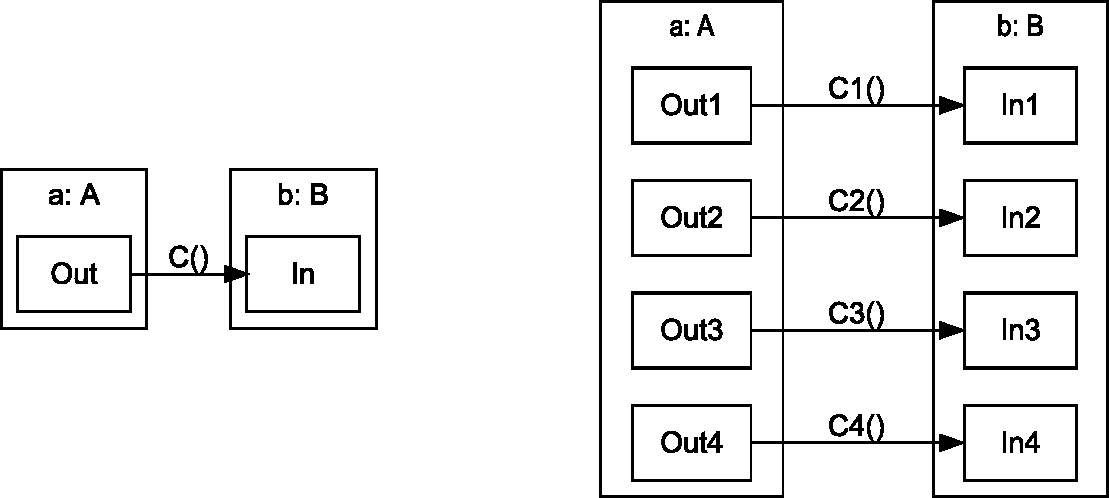
\includegraphics[scale=0.45]{slco/figs/transformations/ExclusiveChannels_Communication}
  \caption{Communication before and after adding exclusive channels}
  \label{fig:slco:excomm}
\end{figure}

On the left of Figure~\ref{fig:slco:excomm}, two objects are shown that communicate over a single channel.
Both objects contain two state machines (which are not shown in this type of diagram) that communicate over this channel.
After applying transformation~\Transformation{ex}, the channel is replaced by four channels, as shown on the right of Figure~\ref{fig:slco:excomm}.

\begin{figure}[hbt]
  \centering
  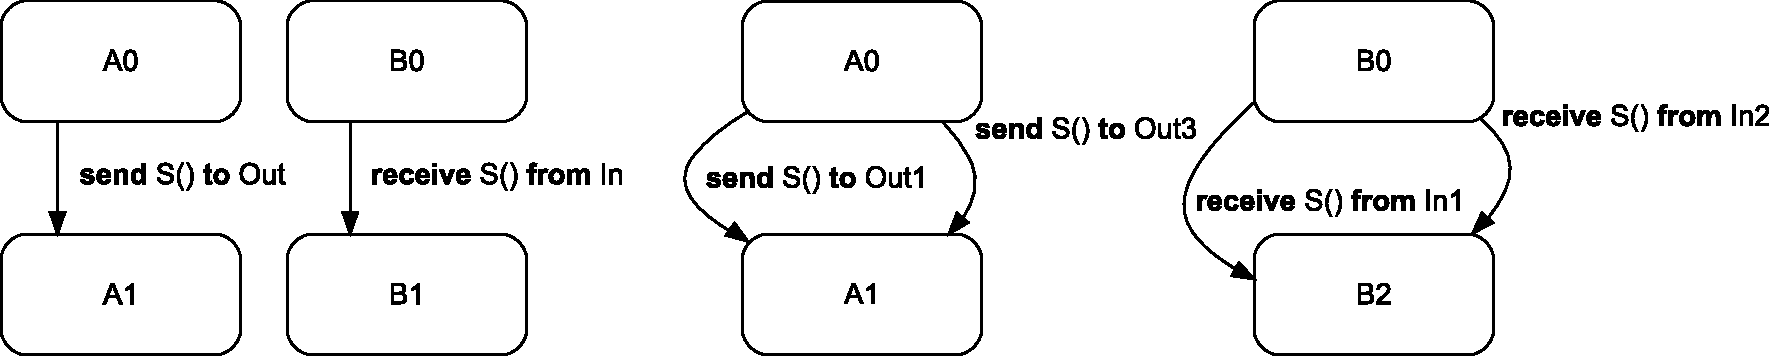
\includegraphics[scale=0.45]{slco/figs/transformations/ExclusiveChannels_Behavior}
  \caption{State machines before and after adding exclusive channels}
  \label{fig:slco:exsm}
\end{figure}

As a part of the process of replacing a channel by multiple channels, transformation~\Transformation{ex} modifies the state machines that communicate over these channels.
Before transformation, both state machines that are part of object~\SLCOObject{a} send signals via port~\SLCOPort{Out}, and both state machines that are part of object~\SLCOObject{b} receive signals via port~\SLCOPort{In}.
After transformation, one of the state machine of object~\SLCOObject{a} sends signals via ports~\SLCOPort{Out1} and~\SLCOPort{Out3}, and the other uses ports~\SLCOPort{Out2} and~\SLCOPort{Out4}.
The receiving state machines are modified in a similar fashion.
Figure~\ref{fig:slco:exsm} shows parts of one of the state machine of object~\SLCOObject{a} and parts of one of the state machines of object~\SLCOObject{b} before and after transformation.
The names of the states of these partial state machines correspond to the names of the classes they belong to.
The situation before transformation is illustrated on the left of the figure, and the situation after transformation is shown on the right.
%Before transformation, as shown on the left of the figure, state~\SLCOState{A0} has only one outgoing transition.
%When making this transition from state~\SLCOState{A0} to state~\SLCOState{A1}, a signal is sent via port~\SLCOPort{Out}.
%State~\SLCOState{B0} also has only one outgoing transition before transformation.
%When a signal is received via port~\SLCOPort{In}, the transition to state~\SLCOState{B1} is made.


\subsubsection{Reducing the Number of Channels}
When two objects are connected by more than one channel, these channels can be merged into one if they have the same type and directionality, and support the same argument types.
Therefore, we implemented a transformation~\Transformation{mc} that merges multiple channels between a pair of objects into one channel.
Merging channels is a way of optimizing models because it can be used to reduce the number of instances of the CABP that need to be added.

\subsubsection{Cloning Classes}
Many of the transformations described above use two auxiliary transformations.
One of these transformations takes a model and a channel as input, and clones the classes of the objects that communicate over this channel.
After applying this transformation, the objects that communicate over the channel are instances of the new cloned classes, and all remaining instances of the original classes remain unchanged.
This transformation ensures that all transformations that alter objects that communicate over a certain channel only affect these particular objects.

\begin{figure}[hbt]
  \centering
  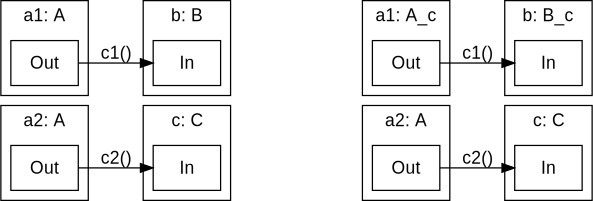
\includegraphics[scale=0.45]{slco/figs/transformations/CloneClasses}
  \caption{A model before and after cloning classes}
  \label{fig:slco:clone}
\end{figure}

Figure~\ref{fig:slco:clone} shows the communication diagram of a model before and after applying this transformation.
After transformation, the classes of the objects communicating over channel~\SLCOChannel{c1} are cloned.
In the resulting model, object~\SLCOObject{a1} is an instance of class~\SLCOClass{A\_c} and object~\SLCOObject{b} an instance of class~\SLCOClass{B\_c}.

\subsubsection{Removing Unused Classes}
The second auxiliary transformation used by the transformations described above removes all uninstantiated classes from a model.
The model depicted on the right of Figure~\ref{fig:slco:clone}, for example, no longer contains an instance of class~\SLCOClass{B}, which means that this class can be removed without affecting the system specified by the model.

%These two transformations are not shown in Figure~\ref{fig:TransformationSequences} to increase its readability.

%%%%%%%%%%%%%%%%%%%%%%%%%%%%%%%%%%%%%%%%%%%%%%%%%%%%
%%%%%%%%%%%%%%%%%%%%%%%%%%%%%%%%%%%%%%%%%%%%%%%%%%%%
%%%%%%%%%%%%%%%%%%%%%%%%%%%%%%%%%%%%%%%%%%%%%%%%%%%%
%%%%%%%%%%%%%%%%%%%%%%%%%%%%%%%%%%%%%%%%%%%%%%%%%%%%




\subsection{Exogenous Transformations}
\label{sec:slco:exogenous}
Each of the following exogenous model transformations takes an \SLCO model as input and produces a model or an implementation in one of the target languages.
Because of the gaps described in Section~\ref{sec:slco:language-gaps}, the \SLCO model provided as input must be specified using a subset of \SLCO that matches the capabilities of the target language and platform.
Any model that is specified using constructs that have no direct counterparts in the target language must first be refined using the transformations described in Section~\ref{sec:slco:endogenous}.

\subsubsection{Transforming \SLCO to \POOSL}
\label{sec:slco:transformation-to-poosl}

\begin{listing}
  \lstset{
    language=poosl,
    label=lst:slco:POOSLModel,
    caption=Part of a \POOSL model,
    numbers=left
  }
  \begin{lstlisting}
    ...
    process class P()
      instance variables m: Integer, PSendRecs: String
      communication channels In1, In2, InOut
      message interface InOut?T(String); In2?Q(Integer); ...
      initial method call P_initial()()
      instance methods
        P_initial()() | |
          m := 0; par Rec1_Rec1()() and Rec2_Rec2()() and SendRec_SendRec()() rap
        .
        Rec1_Rec1()() | var_1: Boolean |
          In1?P(var_1 | var_1 = false); Rec1_Rec1()()
        .
        SendRec_SendRec()() | |
          [m = 6] skip; InOut!S("a"); InOut?T(PSendRecs); SendRec_SendRec()()
        .
    ...
        Com_Com0()() | |
          sel delay(5) or Out1!P(true); Com_Com1()() les
        .
    ...
    behaviour specification
      (p: P[c3/InOut, c1/In1, c2/In2] || q: Q[c1/Out1, c2/Out2, c3/InOut])
      \ {c1, c2, c3}
    .
  \end{lstlisting}
\end{listing}

Because of the gaps between \SLCO and \POOSL, the transformation from \SLCO to \POOSL is restricted to models that contain only synchronous channels.
An example of the output of this transformation is shown in Listing~\ref{lst:slco:POOSLModel}.
This fragment of a \POOSL model is the result of applying the transformation to a slightly modified version of the model of Figures~\ref{fig:slco:SLCOExampleCommunication}, \ref{fig:slco:SLCOExampleStructure}, and~\ref{fig:slco:SLCOExampleSMS}.
The model has been modified by replacing all asynchronous channels by synchronous channels.

The transformation transforms each \SLCO class to a \POOSL process class.
Lines~2 to~16 of Listing~\ref{lst:slco:POOSLModel} show the process class that represents the \SLCO class~\SLCOClass{P}.
The state machines of each class are transformed to a number of process methods, one for each state.
The method in lines~11 to~13 represents the state~\SLCOState{Rec1}, the method in lines~14 to~16 represents the state~\SLCOState{SendRec}, and the method in lines~18 to~20 represents the state~\SLCOState{Com0}.
Besides this, an additional process method is generated for each class, which calls all process methods representing the initial states of the state machines of the class.
These additional process methods also initialize the variables of the classes and state machines to their initial values, if applicable.
Lines~8 to~10 show the process method that initializes the variable~\SLCOVariable{m} of class~\SLCOClass{P} and calls the process methods that represent the initial states of its state machines as part of a parallel composition.

Since each \SLCO class corresponds to exactly one \POOSL process class, it is clear that the global variables of an \SLCO class can be represented by variables of the corresponding \POOSL class.
An \SLCO state machine, however, is represented by multiple process methods, and a group of process methods within a process class cannot share variables that are inaccessible by other process methods of that class.
For this reason, the local variables of \SLCO state machines have to be represented by variables of process classes too.
These variables can no longer be considered to be local to a certain state machine, since all the process methods of a class can access them, even those representing other state machines of the same class.
Line~3 shows the declaration of the \POOSL variables representing the global \SLCO variable~\SLCOVariable{m} and the local \SLCO variable~\SLCOVariable{s} of state machine~\SLCOStateMachine{SendRec}.

States with a single outgoing transition are translated to process methods containing a single sequence of statements.
This sequence of statements represents the outgoing transition.
Line~12 shows the sequence of statements representing the outgoing transition of state~\SLCOState{Rec1}, and line~15 shows the sequence of statements representing the outgoing transition of state~\SLCOState{SendRec}.

States with multiple outgoing transitions are translated to process methods containing a select statement.
Each of the alternatives of such a select statement represents one of the outgoing transitions.
Line~19 shows the select statement representing the outgoing transitions of state~\SLCOState{Com0}.
The semantics of the \POOSL select statement is as follows.
Each of the alternatives of a select statement is a sequence of statements.
If one or more of these sequences starts with a statement that is enabled, one of these sequences is chosen non-deterministically and executed.
If none of the statements are enabled, the select statement is blocked until one of the statements it contains becomes enabled.

As mentioned above, each transition is transformed to a sequence of statements.
If a transition leads to an ordinary state, the sequence of statements representing this transition ends with a process method call.
This process method call calls the method representing the target state of the transition.
Line~12 shows the sequence of statements that represents the transition from state~\SLCOState{Rec1} to itself.
If a transition leads to a final state, this process method call is omitted.
The first alternative of the select statement on line~19 shows an example of this situation.
After 5~ms, the method representing state~\SLCOState{Com0} terminates.

\POOSL does not offer the form of conditional signal reception that uses expressions as arguments to limit the types of signals that can be received.
For this reason, auxiliary variables are introduced to mimic this form of conditional signal reception.
Lines~11 and~12 show how variable~\POOSLVariable{var\_1} is used to do so.

Lines~23 and~24 show that objects~\SLCOObject{p} and~\SLCOObject{q} are declared to be instances of classes~\SLCOClass{P} and~\SLCOClass{Q}, and that channels~\SLCOChannel{c1}, \SLCOChannel{c2}, and~\SLCOChannel{c3} are connected to the ports of these objects.

%%%%%%%%%%%%%%%%%%%%%%%%%%%%%%%%%%%%%%%%%%%%%%%%%%%%
%%%%%%%%%%%%%%%%%%%%%%%%%%%%%%%%%%%%%%%%%%%%%%%%%%%%
%%%%%%%%%%%%%%%%%%%%%%%%%%%%%%%%%%%%%%%%%%%%%%%%%%%%
%%%%%%%%%%%%%%%%%%%%%%%%%%%%%%%%%%%%%%%%%%%%%%%%%%%%



\subsubsection{Transforming \SLCO to \NQC}
\label{sec:slco:transformation-to-nqc}

The transformation from \SLCO to \NQC transforms \SLCO models to \NQC implementations, provided that the following two conditions hold.
First, all objects describing the behavior of the controllers must communicate with each other via asynchronous, lossy channels.
Second, all communication between these objects and the object(s) representing the hardware environment takes place over synchronous channels.

\begin{figure}[hbt]
  \centering
  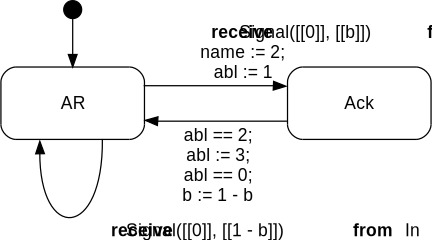
\includegraphics[scale=0.45]{slco/figs/slco2nqc/SimplifiedAR}
  \caption{Part of the Concurrent Alternating Bit Protocol}
  \label{fig:slco:CABP}
\end{figure}

\begin{listing}
  \lstset{
    language=nqc,
    label=lst:slco:NQCCode,
    caption=Fragment of \NQC code,
    numbers=left
  }
  \begin{lstlisting}
    ...
    task AR() {
      int b = 0; int temp;
      AR:
        temp = Message();
        if (
          temp != 0 && ((temp & 112) / 16) == 0 && ((temp & 128) / 128) == b
        ) {
          name = 2; abl = 1; goto Ack;
        }
        temp = Message();
        if (
          temp != 0 && ((temp & 112) / 16) == 0 && ((temp & 128) / 128) == (1 - b)
        ) {
          goto AR;
        }
      goto AR;
      Ack:
        if (abl == 2) {
          abl = 3; /* skip */; until (abl == 0); b = 1 - b; goto AR;
        }
      goto Ack;
    }
  \end{lstlisting}
\end{listing}

Figure~\ref{fig:slco:CABP} shows the state machine of object~\SLCOObject{ar} that is part of the implementation of the CABP introduced in Section~\ref{subsubsec:slco:ll} after merging it with objects~\SLCOObject{a} and~\SLCOObject{sender}.
Listing~\ref{lst:slco:NQCCode} shows a fragment of \NQC code that is the result of applying the transformation from \SLCO to \NQC to a model containing the merged objects.

Every state machine that describes the behavior of an object in an \SLCO model is transformed into an \NQC task.
Lines~2 to~23 show the task that represents the state machine of Figure~\ref{fig:slco:CABP}.
Line~3 shows the declaration and initialization of local variable~\SLCOVariable{b} and auxiliary variable~\NQCVariable{temp}.
The purpose of auxiliary variable~\NQCVariable{temp} is explained below.
Global variables of \SLCO objects, such as~\SLCOVariable{abl} and~\SLCOVariable{name} in Figure~\ref{fig:slco:CABP}, are represented by global variables of \NQC programs, and are not shown in Listing~\ref{lst:slco:NQCCode}.

Each state is represented by a label, followed by sequences of statements that represent the outgoing transitions of the state, and a goto statement that jumps back to the label.
Lines~4 to~17 show the labeled sequence of statements representing state~\SLCOState{AR}, and lines~18 to~22 represent state~\SLCOState{Ack}.

If the statements of an \SLCO transition start with a statement that might block execution, this statement is translated to an \NQC if statement and the remaining \SLCO statements are translated to \NQC statements that form the body of this if statement.
In case the first statement is a signal reception statement, the if statement is preceded by a call to the API function~\NQCFunction{Message}.
The purpose of this API call is explained below.
Lines~5 to~10,~11 to~16, and~19 to~21 represent the transitions of the state machine in Figure~\ref{fig:slco:CABP}.
The remaining statements that are part of an \SLCO transition are translated as follows.
Assignments in \SLCO are translated to assignments in \NQC, as shown in lines~9 and~20.
Expressions and signal receptions are translated to until statements, as shown in line~20.
Statements that send signals are not shown in this example.
They are translated to calls to the API function~\NQCFunction{SendMessage}, using the encoding explained below.

An RCX controller can only send and receive integer values over its infrared port.
Since signals in \SLCO consist of a name and possibly a number of arguments, they have to be encoded such that they can be represented as a single integer before they can be sent, and they have to be decoded after being received.
Lines~5 and~11 show that first the auxiliary variable~\NQCVariable{temp} is used to store the value of the integer that has been received last.
Then, this integer is decoded as shown in lines~7 and~13.
The encoding of a signal, which is not shown in this example, is done using a similar procedure.
The actual sending and receiving of integer values is done via API calls to the functions~\NQCFunction{Message} and~\NQCFunction{SendMessage}, as mentioned above.

In addition to an \SLCO model, the transformation from \SLCO to \NQC also takes a mapping from elements in the \SLCO model to concepts of \NQC as input.
Listing~\ref{lst:slco:SLCO2NQCMapping} shows a part of the mapping for the model described in Section~\ref{sec:slco:sequences}.
For each class that needs to be transformed to an \NQC program, this mapping defines how some of the signals of an \SLCO model correspond to information received from sensors and commands sent to motors.
Each signal that is not mentioned in this mapping is assumed to be part of the communication between controllers via infrared and is translated accordingly, as described above.

\begin{listing}
  \lstset{
    language=slco2nqc,
    label=lst:slco:SLCO2NQCMapping,
    caption=Part of a mapping from \SLCO to \NQC,
    numbers=left
  }
  \begin{lstlisting}
    class Middle
      port2motor
        Motor -> OutB 7
      port2sensor
        Sensor -> Sensor2 Light
      signal2motor
        Motor Left -> On Reverse
        Motor Right -> On Forward
        Motor Off -> Float
      signal2sensor
        Sensor Block -> Below -10
        Sensor BlockPassed -> Above -2
  \end{lstlisting}
\end{listing}

In line~3, port~\SLCOPort{Motor} of an \SLCO model is mapped to output port~\NQCPort{OutB} of a Lego Mindstorms controller.
The speed of the motor is set to 7.
In line~5, \SLCO port~\SLCOPort{Sensor} is mapped to input port~\NQCPort{Sensor2} of a Lego Mindstorms controller, which is connected to a light sensor.
Signals named~\SLCOSignalName{Left}, \SLCOSignalName{Right}, and~\SLCOSignalName{Middle} sent over port~\SLCOPort{Motor} are mapped to commands for a motor in lines~7 to~9.
Lines~11 and~12 show how signals named~\SLCOSignalName{Block} and~\SLCOSignalName{BlockPassed} are mapped to information received from sensors.
In line~11, for example, receiving a signal named~\SLCOSignalName{Block} is mapped to the event that the value transmitted by the sensor connected to port~\NQCPort{Sensor2} drops below $-10$.

\subsubsection{Transforming SLCO to Promela}
\label{subsubsec:slco:transformation-to-promela}

The transformation from \SLCO to \Promela transforms \SLCO models containing only synchronous channels and asynchronous, lossless channels to \Promela models.
Listing~\ref{lst:slco:PromelaModel} shows a fragment of a \Promela model that is the result of applying this transformation to a slightly modified version of the \SLCO model described in Figures~\ref{fig:slco:SLCOExampleCommunication}, \ref{fig:slco:SLCOExampleStructure}, and~\ref{fig:slco:SLCOExampleSMS}.
Because \Promela does not support the more general form of conditional signal reception, the condition~$\SLCOVariable{m} \geqop 0$ is removed from the signal reception in the \SLCO model.
Additionally, the asynchronous, lossy channel is replaced by an asynchronous, lossless channel.

\begin{listing}
  \lstset{
    language=promela,
    label=lst:slco:PromelaModel,
    caption=Part of a \Promela model,
    numbers=left
  }
  \begin{lstlisting}
    mtype {S, P, Q, T, a}
    int p_m = 0
    chan c1_q2p = [1] of {mtype, bool}
    chan c3_1_q2p = [0] of {mtype, mtype}
    chan c3_2_q2p = [0] of {mtype, mtype}
    ...
    active [1] proctype p_Rec1() {
      Label_Rec1: {
        if :: {c1_q2p?P,eval(false); goto Label_Rec1} fi
      }
    }

    active [1] proctype p_Rec2() {
      Label_Rec2: {
        if :: {c2_q2p?Q,p_m; p_m = p_m + 1; goto Label_Rec2} fi
      }
    }
    ...
    active [1] proctype q_Com() {
      mtype q_s;
      Label_Com0: {
        if :: {skip; goto Label_Com2}
           :: {c1_q2p!P,true; goto Label_Com1}
        fi
      }
      Label_Com1: {
        if ::
          {c2_q2p!Q,5; c3_1_p2q?S,q_s; c3_2_q2p!T,q_s; goto Label_Com2}
        fi
      }
      Label_Com2: skip
    }
  \end{lstlisting}
\end{listing}

For each object in an \SLCO model, the state machines that describe its behavior are transformed to \Promela processes.
Lines~7 to~11 in Listing~\ref{lst:slco:PromelaModel} show the process that represents state machine~\SLCOStateMachine{Rec1} of object~\SLCOObject{p}, lines~13 to~17 show the process that represents state machine~\SLCOStateMachine{Rec2} of object~\SLCOObject{p}, and lines~19 to~32 show the process that represents state machine~\SLCOStateMachine{Com} of object~\SLCOObject{q}.

Channels between objects in \SLCO are transformed to channels between processes in \Promela.
Line~3 shows the declaration of the \Promela channel representing the \SLCO channel named~\SLCOChannel{c1}.
The 1 between square brackets indicates that this channel is asynchronous.
The declaration specifies that this channel is suited for messages consisting of two parts: a symbolic name (mtype) and a Boolean value.
Lines~4 and~5 show the declaration of two channels representing the \SLCO channel named~\SLCOChannel{c3}.
Although \Promela offers bidirectional channels, a separate channel is declared for each direction.
This is done because the semantics of channels in \Promela differs from their semantics in \SLCO.
In \SLCO, an object can only receive signals sent by another object.
In \Promela, however, a process can retrieve a message from a channel that it has sent over this channel itself.
For this reason, we introduce two \Promela channels for each bidirectional \SLCO channel.
Each of the \Promela channels is used only to communicate in one direction, which means that a process uses the channel either to send messages or to receive messages, but not both.
The 0 between square brackets indicates that this channel is synchronous.

The local variables of state machines are represented by local variables of processes, as shown in line~20.
Global variables of \SLCO objects are represented by global variables of the \Promela model.
They are accessible by all processes in the model.
On line~2, global variable~\SLCOVariable{m} of object~\SLCOObject{p} is declared.

Ordinary states are transformed to labeled selection statements, and final states are transformed to labeled skip statements.
Lines~21 to~25 represent state~\SLCOState{Com0} of object~\SLCOObject{q}, lines~26 to~30 represent state~\SLCOState{Com1}, and line~31 represents state~\SLCOState{Com2}.

Every outgoing transition of a state is represented by an alternative of the selection statement that represents this state.
Each of these alternatives ends with a goto statement to the label representing the target state of the transition.
State~\SLCOState{Rec1} of object~\SLCOObject{p} has only one outgoing transition, as shown in line~9.
State~\SLCOState{Com0} of object~\SLCOObject{q} has two outgoing transitions.
The transition to state~\SLCOState{Com2} is shown in line~22, and the transition to state~\SLCOState{Com1} is shown in line~23.

The semantics of the selection statement is such that it will non-deterministically execute one of the alternatives for which the first statement is executable, and it will block if none of these statements are executable.
The statements of a transition are transformed to \Promela statements in a straightforward way.
Expressions and assignments in \SLCO are translated to equivalent expressions and assignments in \Promela, as shown in line~15.
A signal reception is transformed to a receive statement, as shown in line~9.
The receive statement~\PromelaReceive{c1\_q2p}{P,\PromelaEval(\PromelaFalse)} represents the reception of signals named~\SLCOSignalName{P} with an argument that must be equal to~\SLCOFalse.
A \Promela receive statement blocks until it is able to receive a message over a channel.
A send signal statement is transformed to a send statement in a similar fashion, as shown in lines~23 and~28.  